\documentclass[]{article}

\usepackage{graphicx}

%opening
\title{ARTS1422 HW2}
\author{Suting Chen}

\begin{document}

    \maketitle


    \section{Requirements}
    All code has been tested on Chrome and Safari only. They are guaranteed to work with D3.js.v5


    \section{Task 1}
    Dataset: \underline{http://lib.stat.cmu.edu/datasets/boston}
    
    The original dataset is designed to be human-readable instead of python-friendly, so manual formatting is required.
    
    Then we work with the well-formatted data. ($boston.csv$)
    
    We can easily import these algorithms from scipy and process them for rendering.
    \newpage


    \section{Task 2}
    
    Open $main.html$ (with $boston\_MDS.csv$, $boston\_PCA.csv$ and $boston\_TSNE.csv$ in the same directory) in browser.
    
    \begin{figure}[h]
    	\centering
    	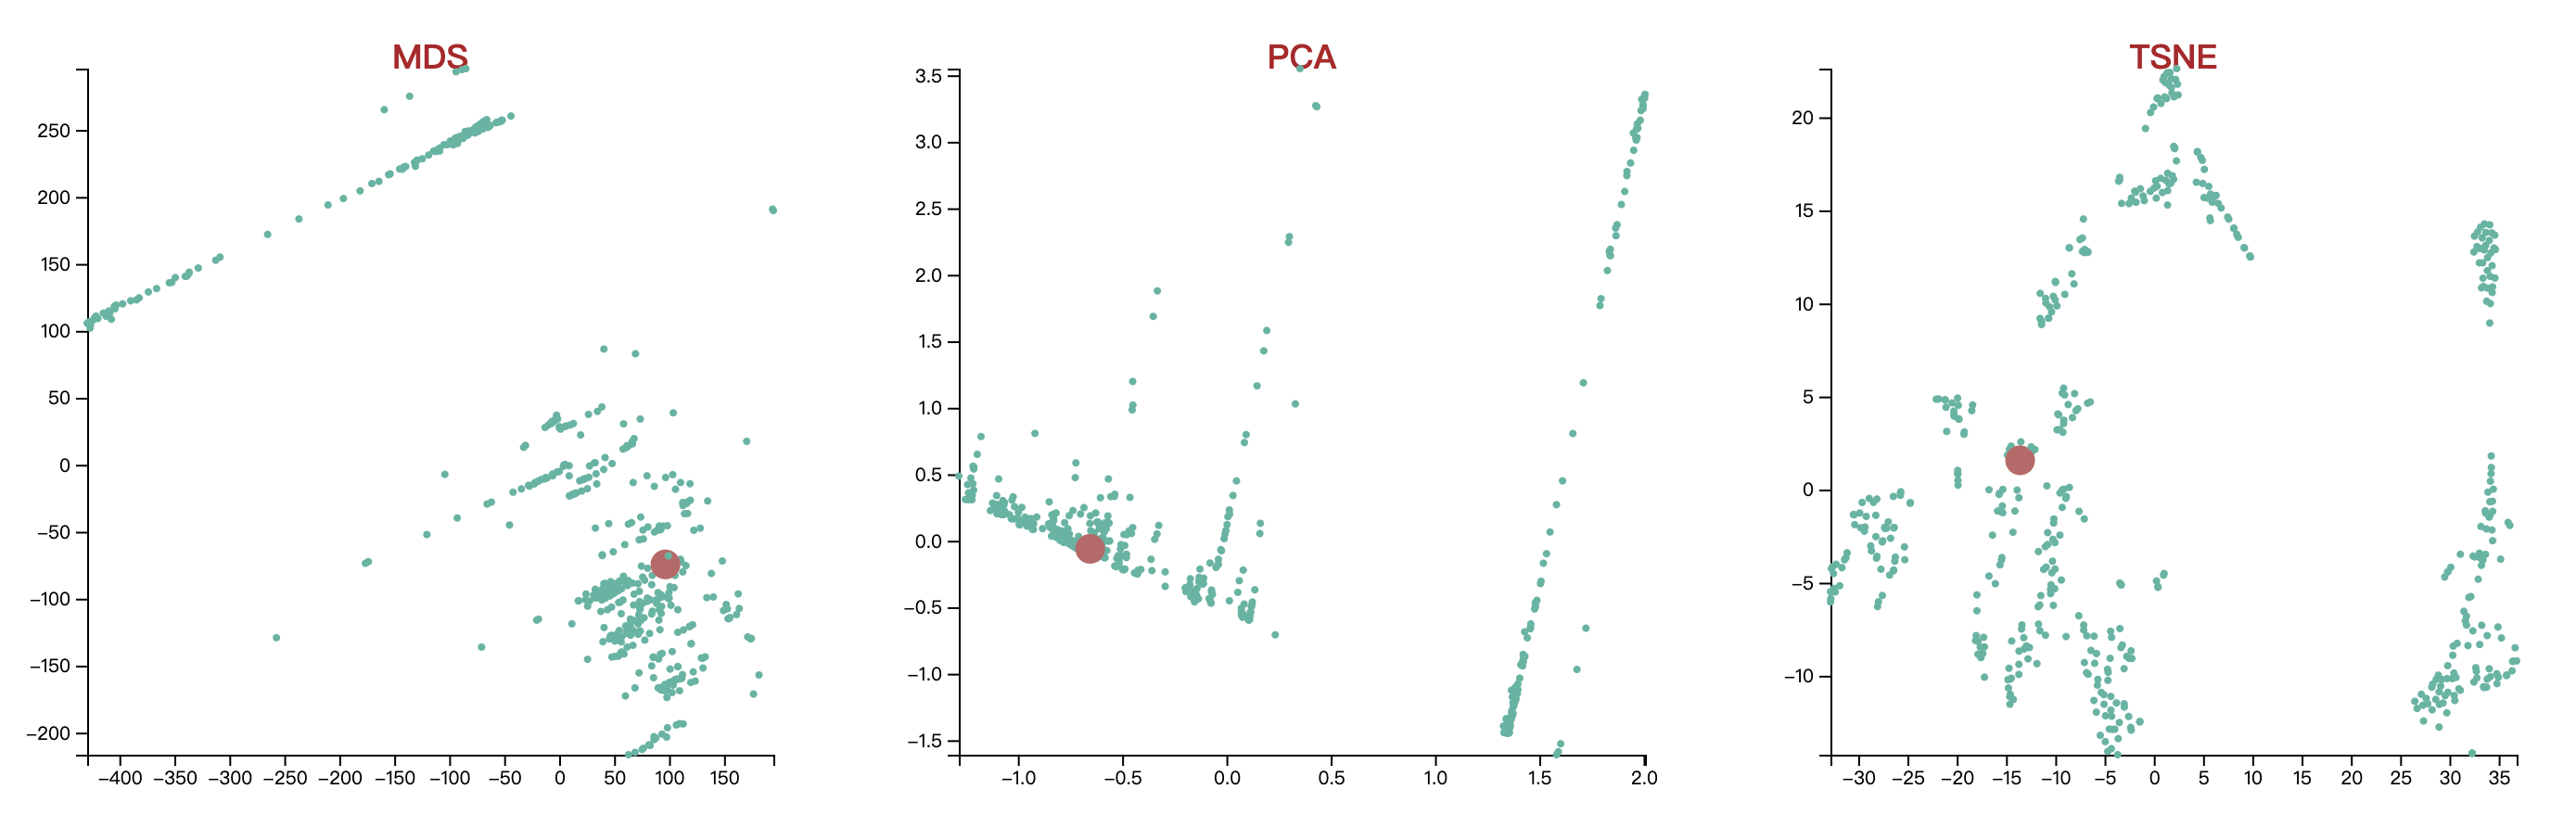
\includegraphics[width=14cm]{task2}
    	\label{fig:task2}
    \end{figure}
    
    As shown above, when mouse hover certain data points, all corresponding points in three graphs is highlighted.
    
    \hspace{3cm}

	\textbf{Evaluation}: A very vital dimension in the dataset is \textbf{AGE}, which means \textbf{proportion of owner-occupied units built prior to 1940}. Only PCA has distinguished them very well, keeping them monotone along with a line in the plot.

\end{document}
